\documentclass[aspectratio=169]{beamer}

\usetheme{metropolis}

% ENCODING AND LANGUAGE
\usepackage[english]{babel}

\usepackage[utf8]{inputenc}     % Universal encoding
\usepackage[T1]{fontenc}        % Font encoding

% FONT
\usepackage{courier}            % Courier as \ttdefault
% \usepackage{psfrag}             % replace PostScript fonts

% OTHER HELPERS AND SETTINGS
% \usepackage{graphicx}           % Include graphics to document
% \usepackage{amsmath,amssymb,amstext}  % support for mathematics ttt

% \usepackage{listings}           % code listings
% \lstset{basicstyle=\footnotesize\ttfamily,breaklines=true}

% \usepackage{units}
\usepackage{siunitx}            % SI-Unit support

% TITLE PAGE SETTINGS
\title{A/V Angel Self-Training: Video Mixer}
% \date{\today \currenttime}
% \author{c3voc}
\institute{C3VOC
	\begin{flushright}
		
\includegraphics[height=0.4\textheight]{images/qr-code.png}\\
		https://github.com/voc/engelschulung
	\end{flushright}
}

%% START OF DOCUMENT
\begin{document}
\maketitle

% \input{selftraining-core.tex}
% !TEX root = ../main.tex

\begin{frame}{General}
	\begin{itemize}
		\item We will stream, record and publish all talks with your help
		\item You can operate the cameras and video mixer
		\item We (people from c3voc) will be there to help
		\item The live stream video signal will also be the final recording
		\item We aim for consistent quality, but everybody make mistakes -- don't blame yourself!
	\end{itemize}
\end{frame}


\section{Video Mixer Tools}
% !TEX root = ../main.tex

\begin{frame}{Software Video Mixer - Voctomix2}
	\begin{figure}
		\centering
		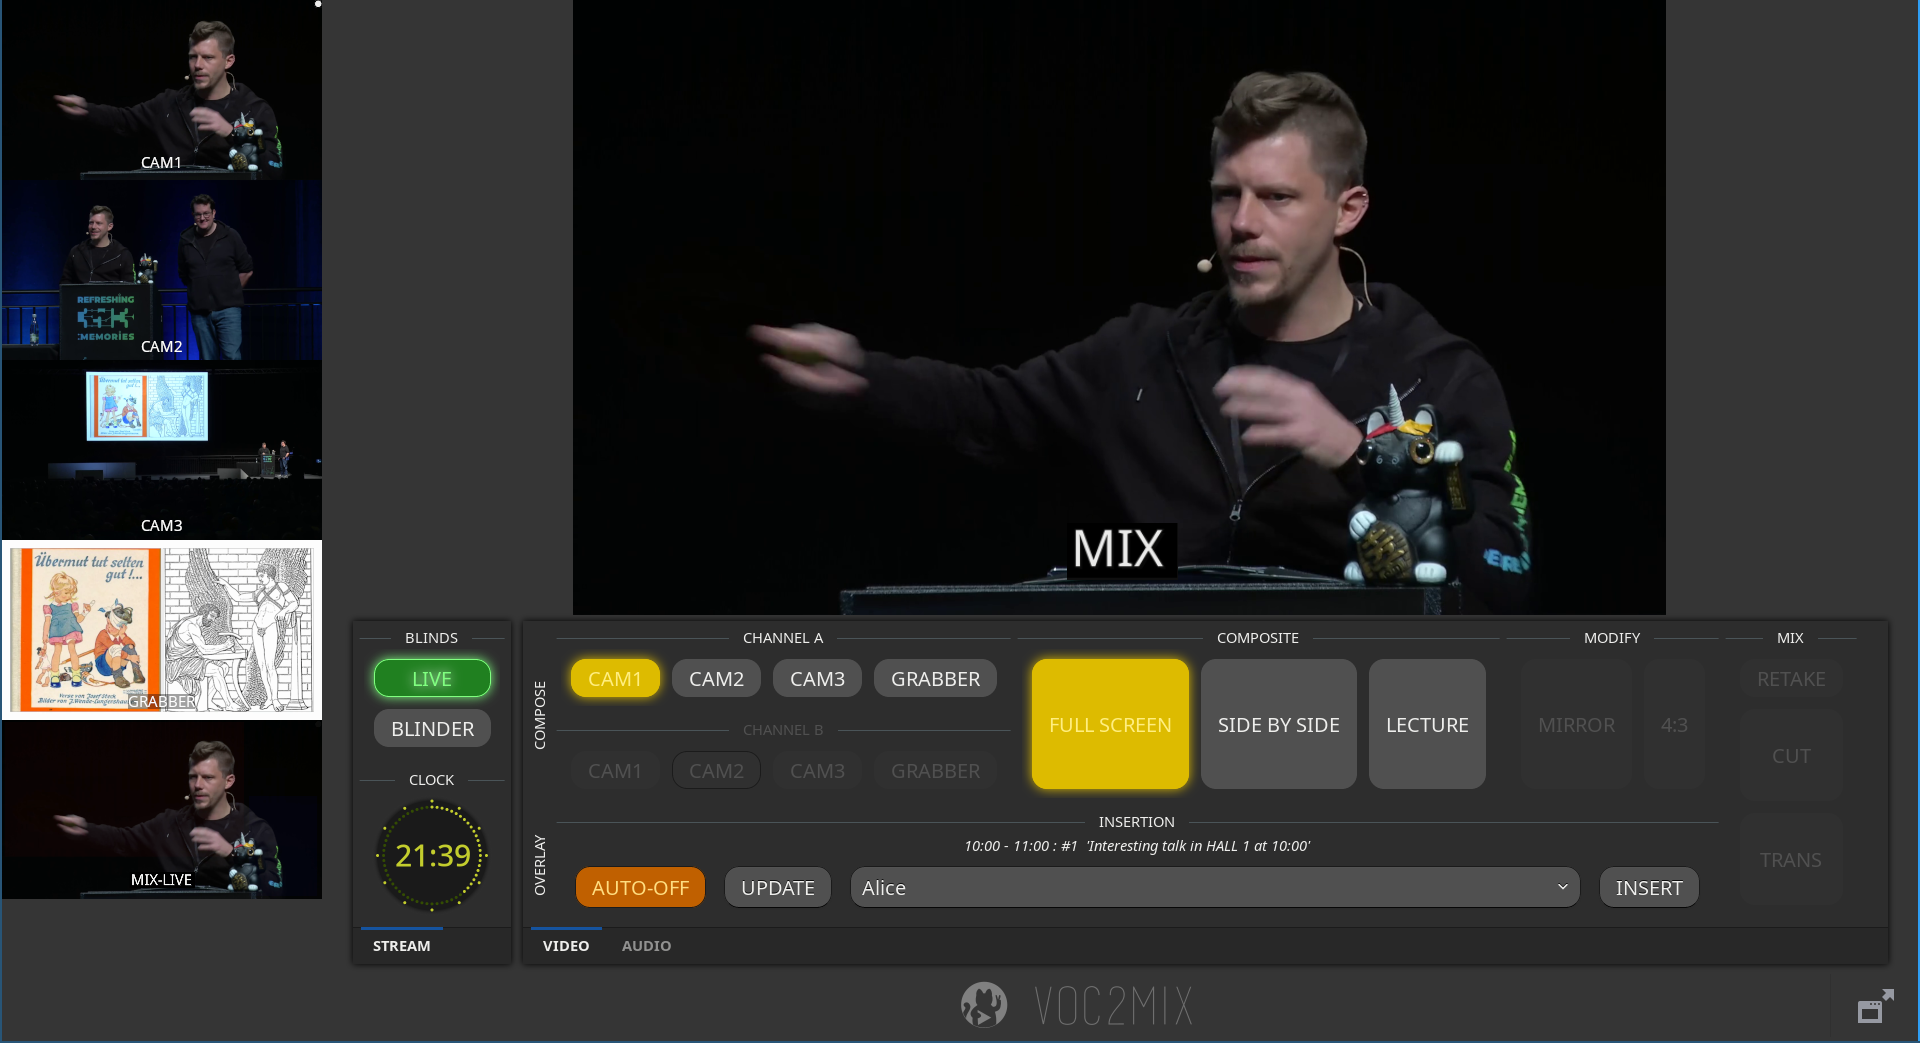
\includegraphics[width=.9\textwidth]{images/voctomix2_1.png}
		\caption{Voctomix2}
	\end{figure}
\end{frame}

\begin{frame}{Software Video Mixer - Voctomix2}
	\begin{figure} 
		\centering
		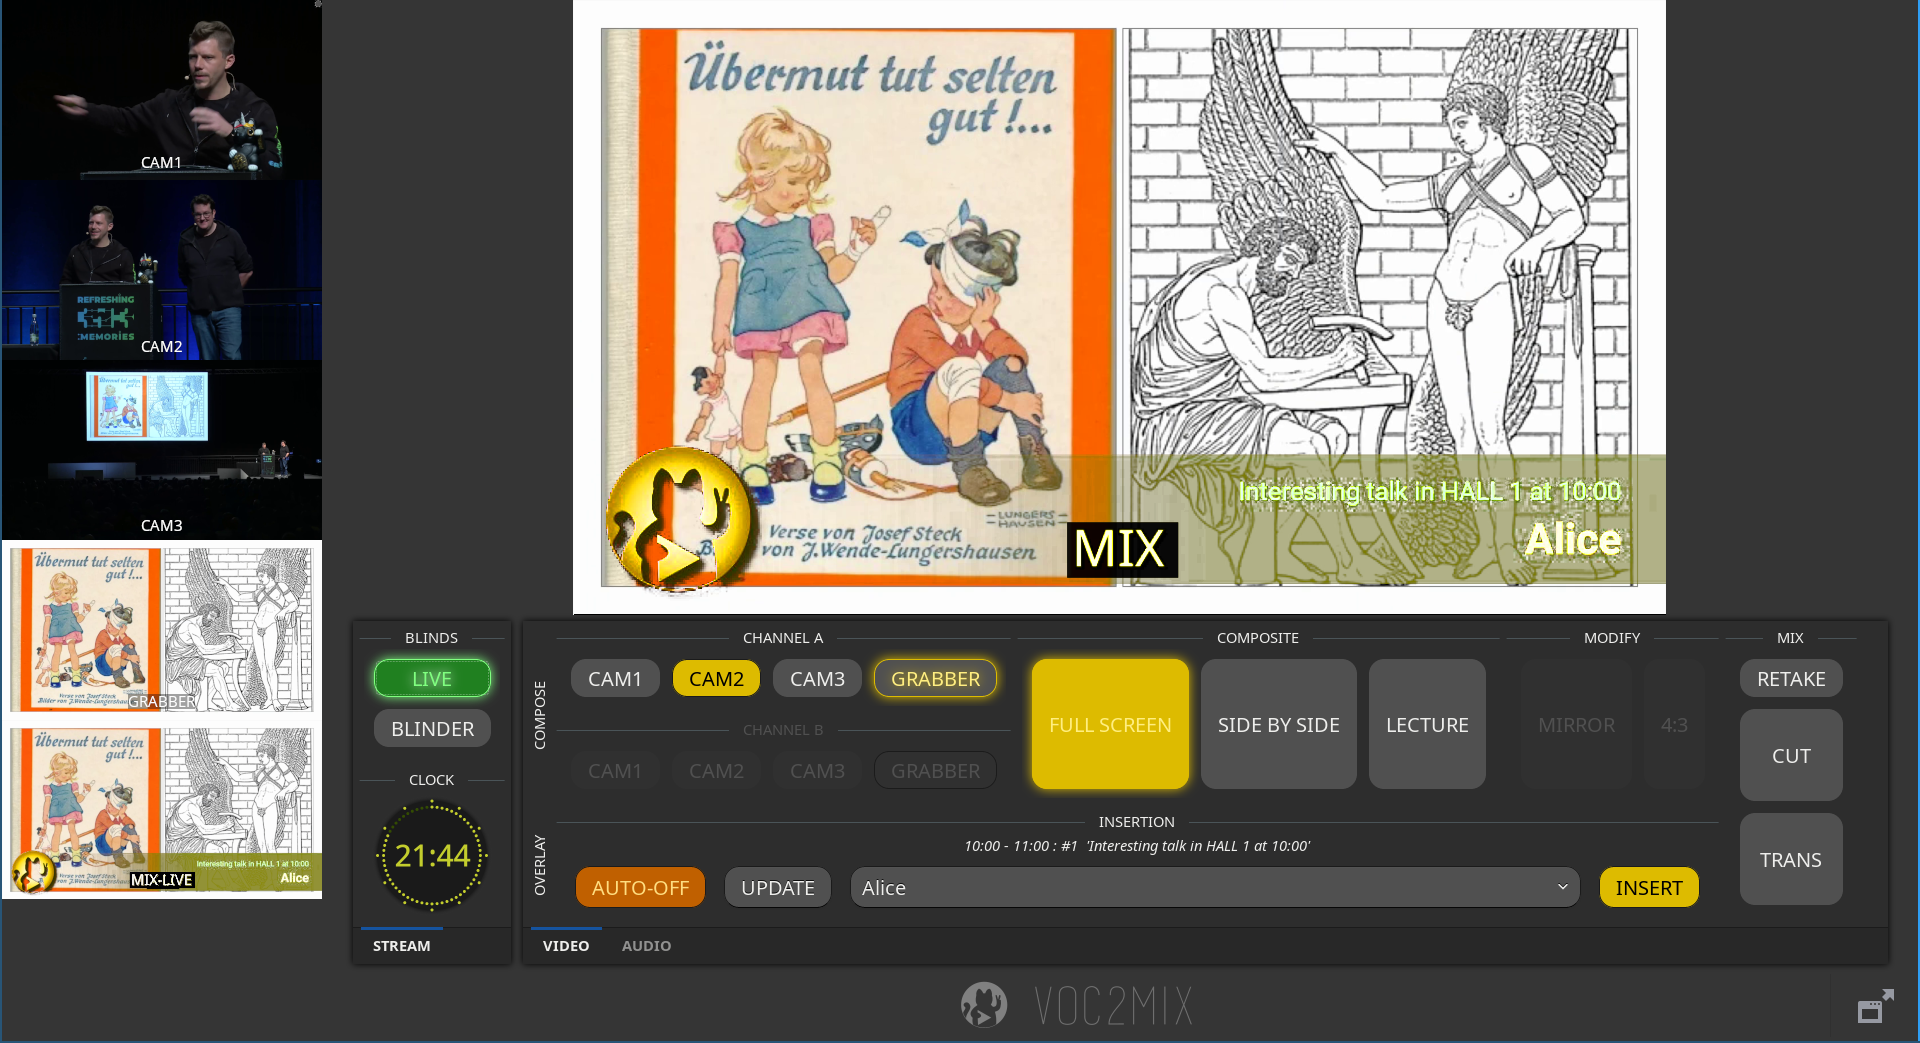
\includegraphics[width=.9\textwidth]{images/voctomix2_2.png}
		\caption{Voctomix2 - Lower Thirds}
	\end{figure}
\end{frame}

\begin{frame}{Software Video Mixer - Voctomix2}
	\begin{figure} 
		\centering
		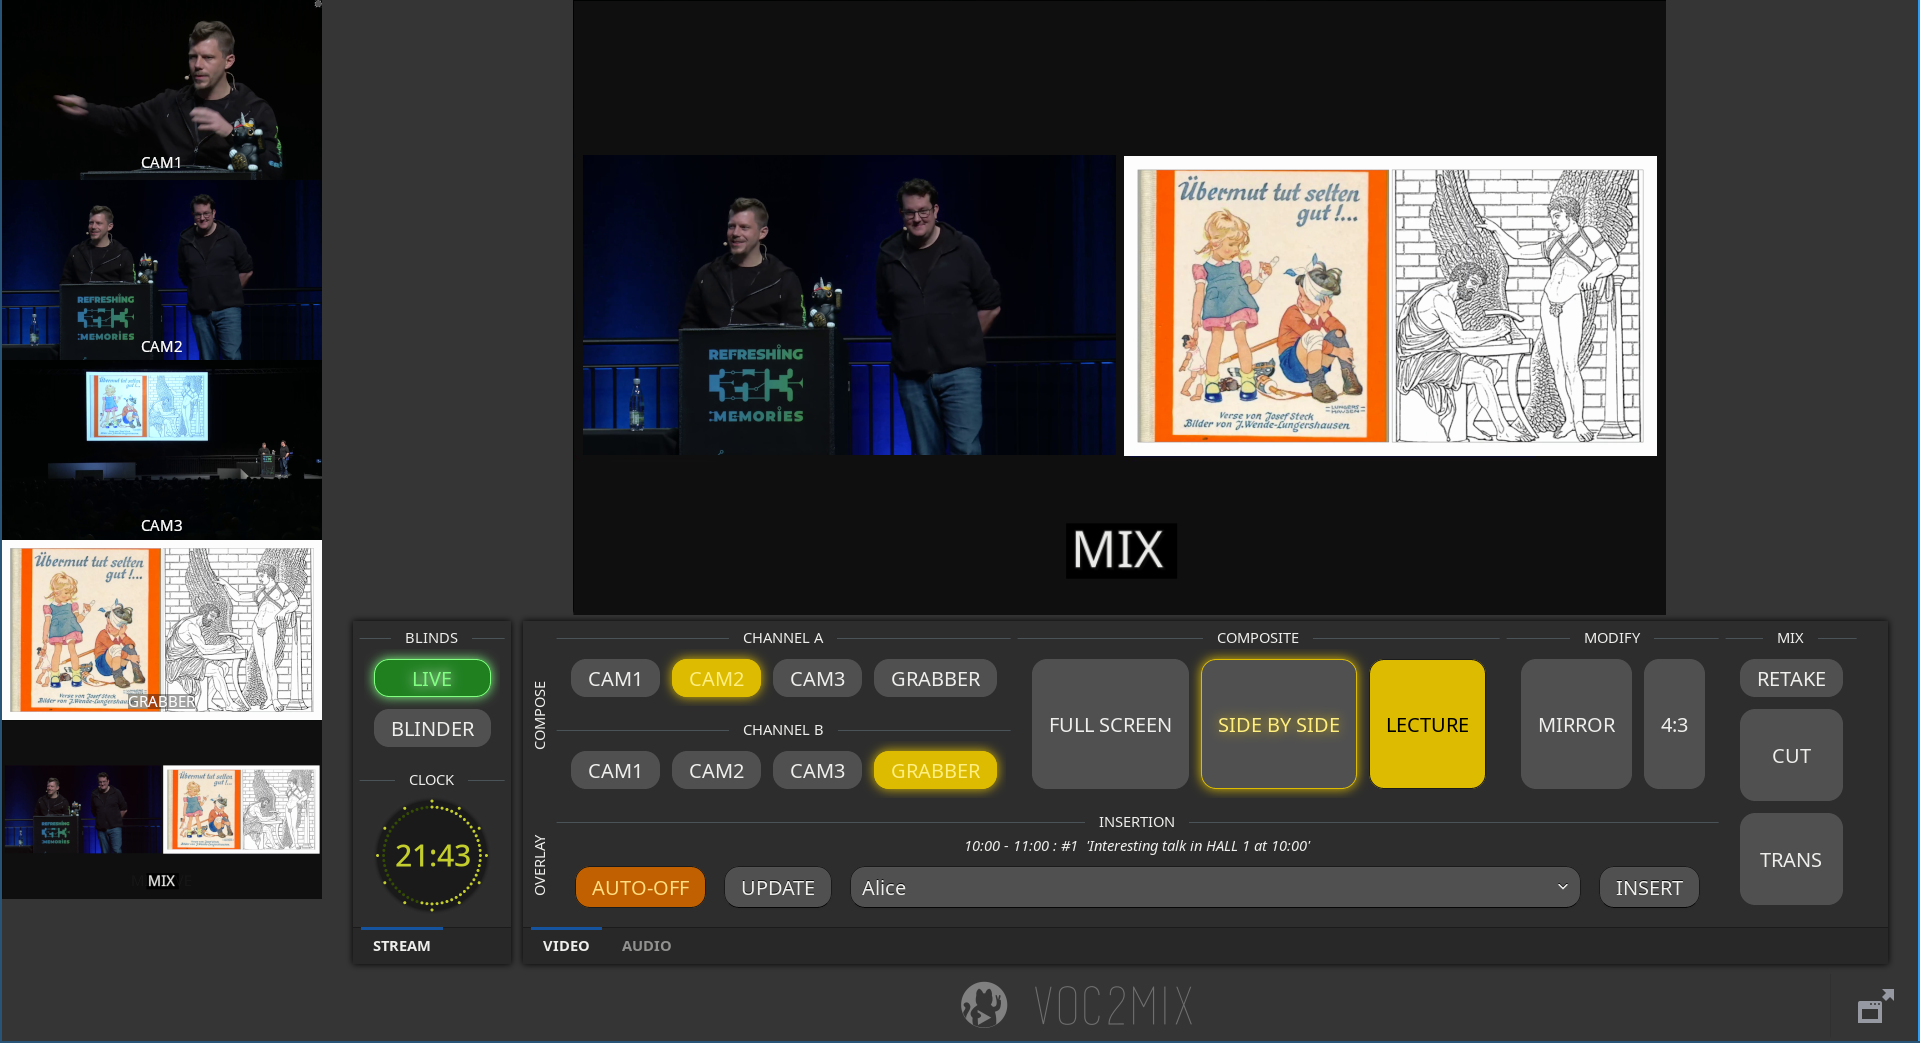
\includegraphics[width=.9\textwidth]{images/voctomix2_3.png}
		\caption{Voctomix2 - Side by Side}
	\end{figure}
\end{frame}


\section{Video Mixing Guidelines}
\begin{frame}{Mixing Guidelines - Hard Rules}
	\begin{itemize}
		\item \textbf{All} you are doing is \textbf{recorded} and will be published. \alert{\textbf{Don't make mistakes.}}
		\item The Audience is \textbf{not to be filmed}. Cut away if faces of people not on the stage appear.
		\item \textbf{Slides are important}
		\item Slides stay on till the text has been read \textbf{twice}.
		\item Show new slides \textbf{immediately}.
	\end{itemize}
\end{frame}

\begin{frame}{Mixing Guidelines - Softer Hints}
	\begin{itemize}
		\item Start early – opening announcements of the Herald are a good start. Their introduction has to be in the recording and on stream.
		\item Open wide – Structure the beginning of a talk with shots that set the stage
		\item The slides in fullscreen – you’re dealing with a very small screen. Text has to be readable
		\item Show gestures – medium-close-up that follows the speakers eye-line
		\item Don’t be too cutty – Pace your videos temperately. Do not cut too often.
		\item Don't end too early – All questions and answers have to be recorded. The herald ends the talk, not the mixer angel.
	\end{itemize}
	\begin{exampleblock}{Hints}
		Leave lots of room at the start and end of a talk. 
		Cut away from the infobeamer before the Herald starts with announcements. 
		Cut to the infobeamer only after the last applause has finished.
	\end{exampleblock}
\end{frame}


\section{Audio Hardware}
% !TEX root = ../main.tex

\begin{frame}{Audio Mixer Controls: Levels}
	\begin{columns}[T,onlytextwidth]
		\column{0.6\textwidth}
		\begin{figure} 
			\centering
			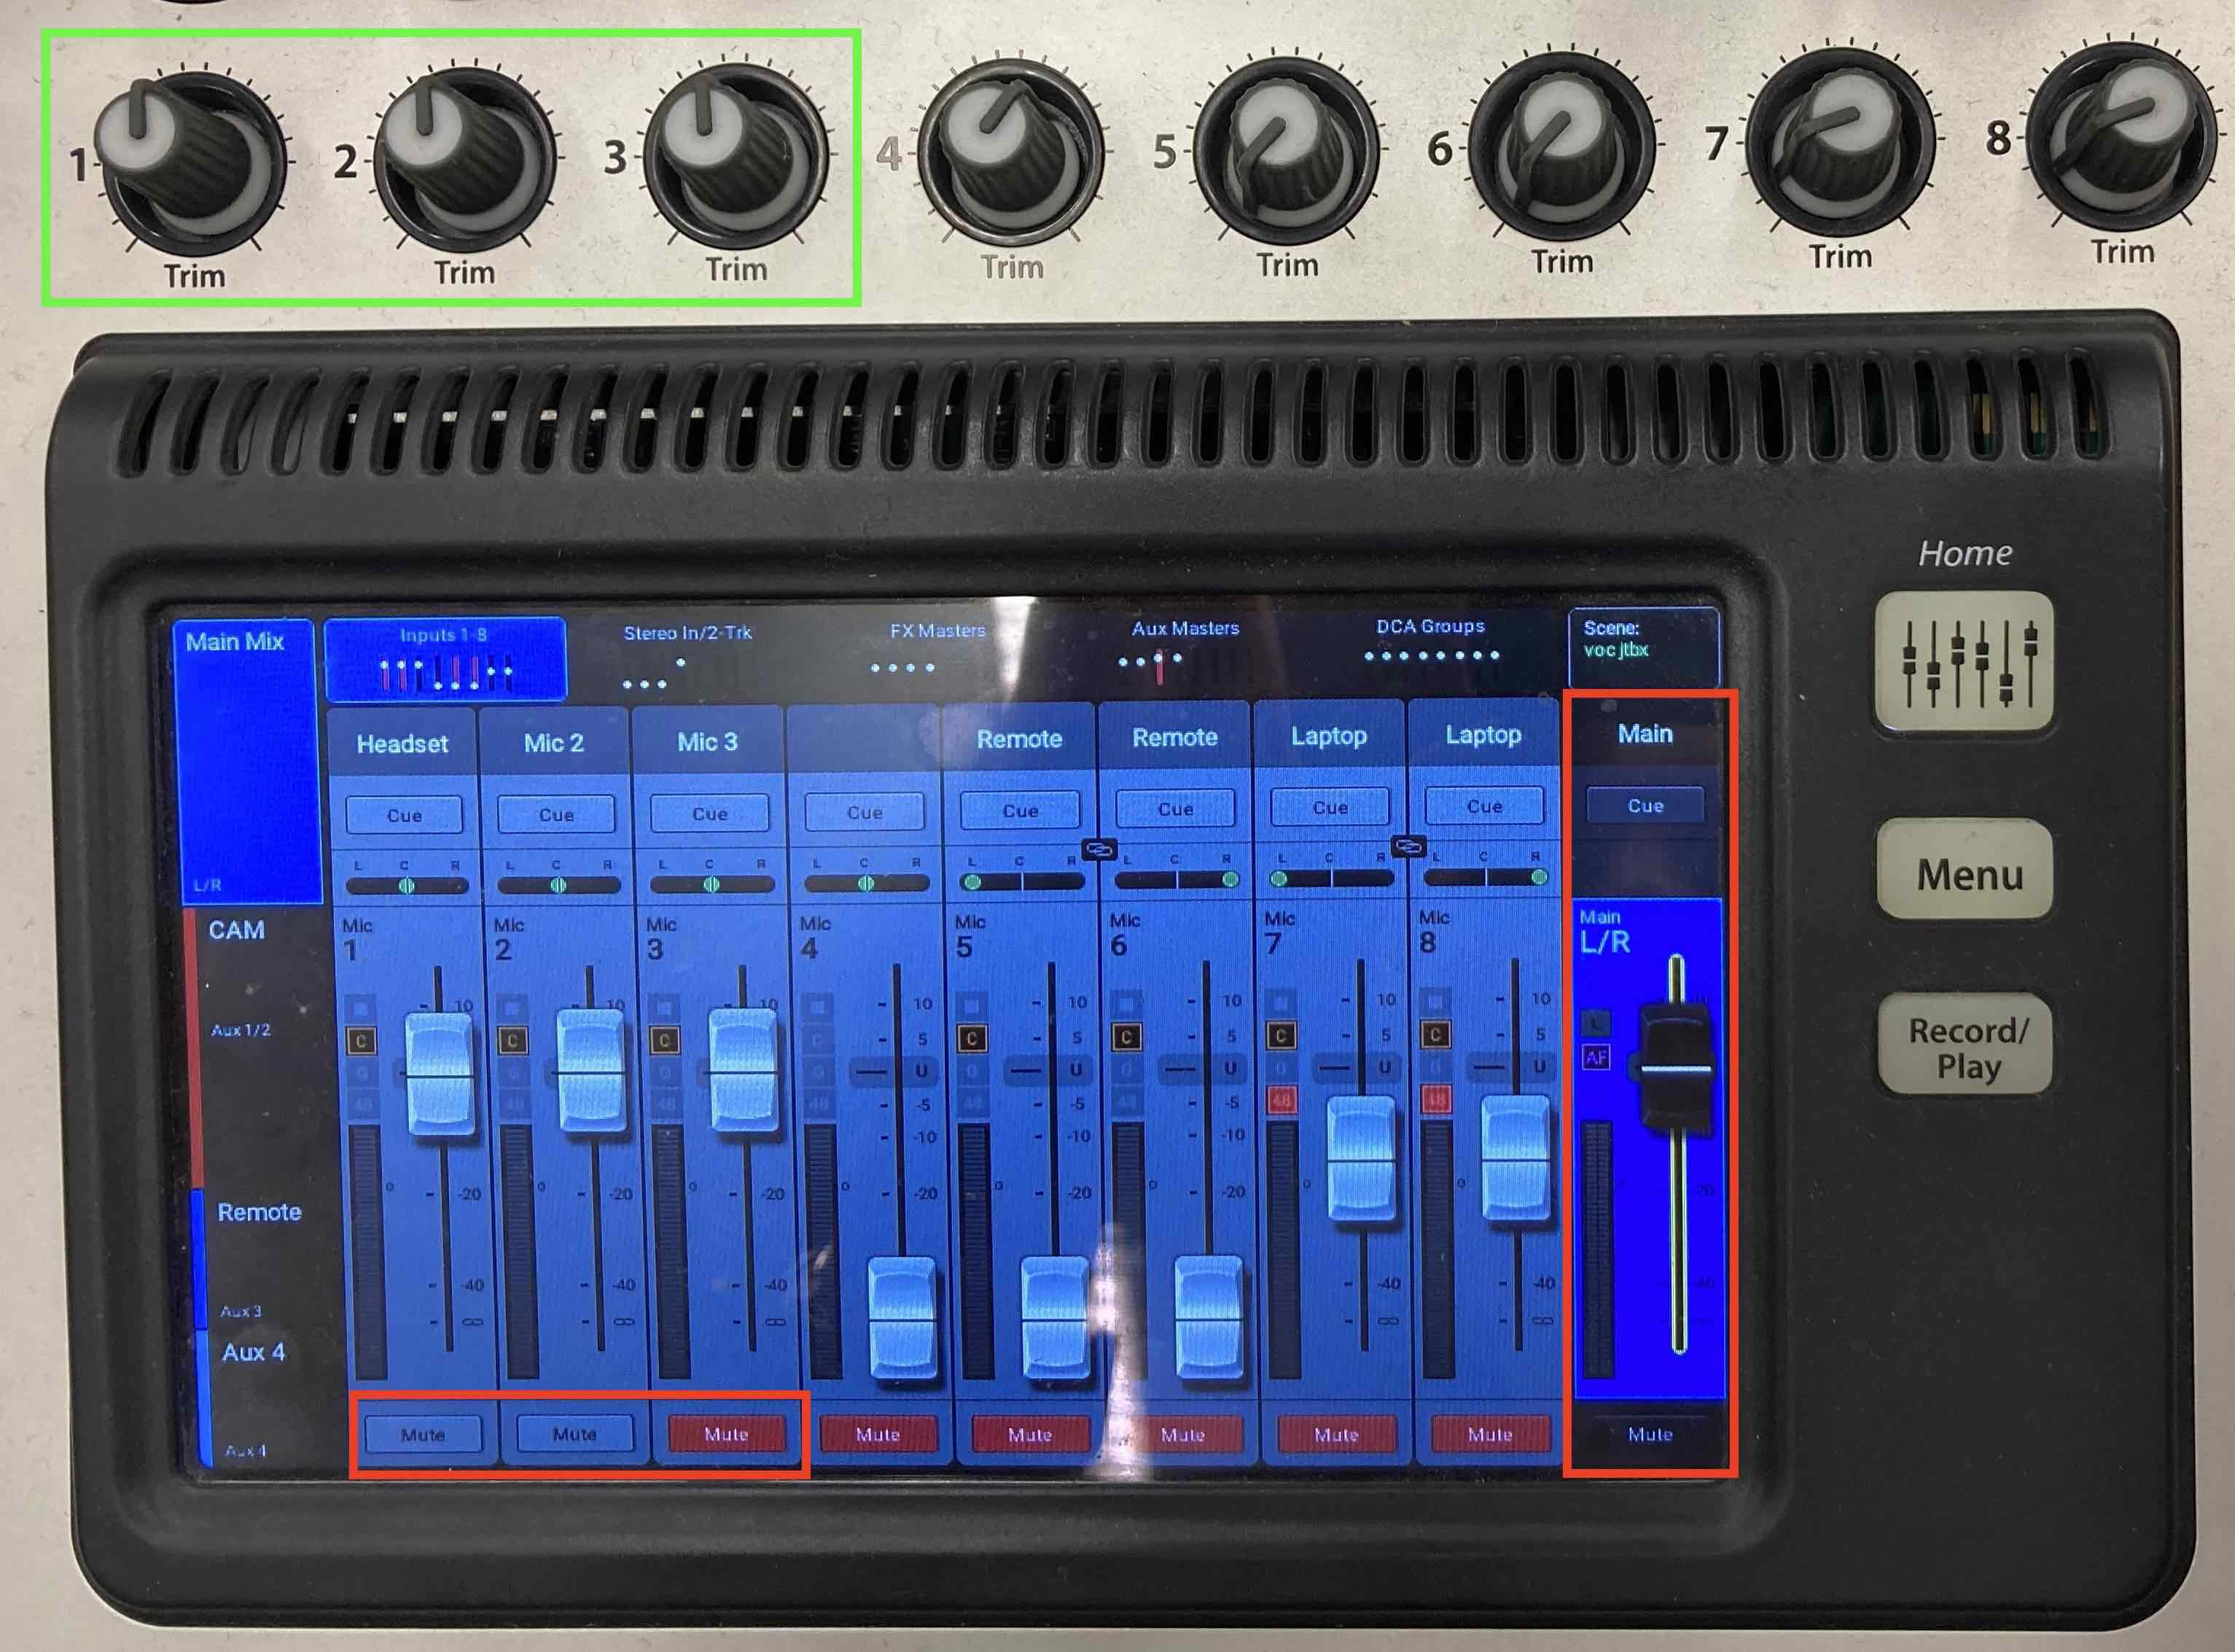
\includegraphics[width=0.9\textwidth]{images/touchmix-main-controls.jpg}
			\caption{Touchmix Main Controls}
		\end{figure}
		\column{0.4\textwidth}
		\begin{itemize}
			\item Mute unused microphones (bottom row)
			\item Adjust hall loudness with rightmost fader
			\item Adjust individual microphone level with fader or redude "trim" knob when it's clipping
		\end{itemize}
	\end{columns}
\end{frame}

\begin{frame}{Audio Mixer Controls: Second Page}
	\begin{columns}[T,onlytextwidth]
		\column{0.6\textwidth}
		\begin{figure} 
			\centering
			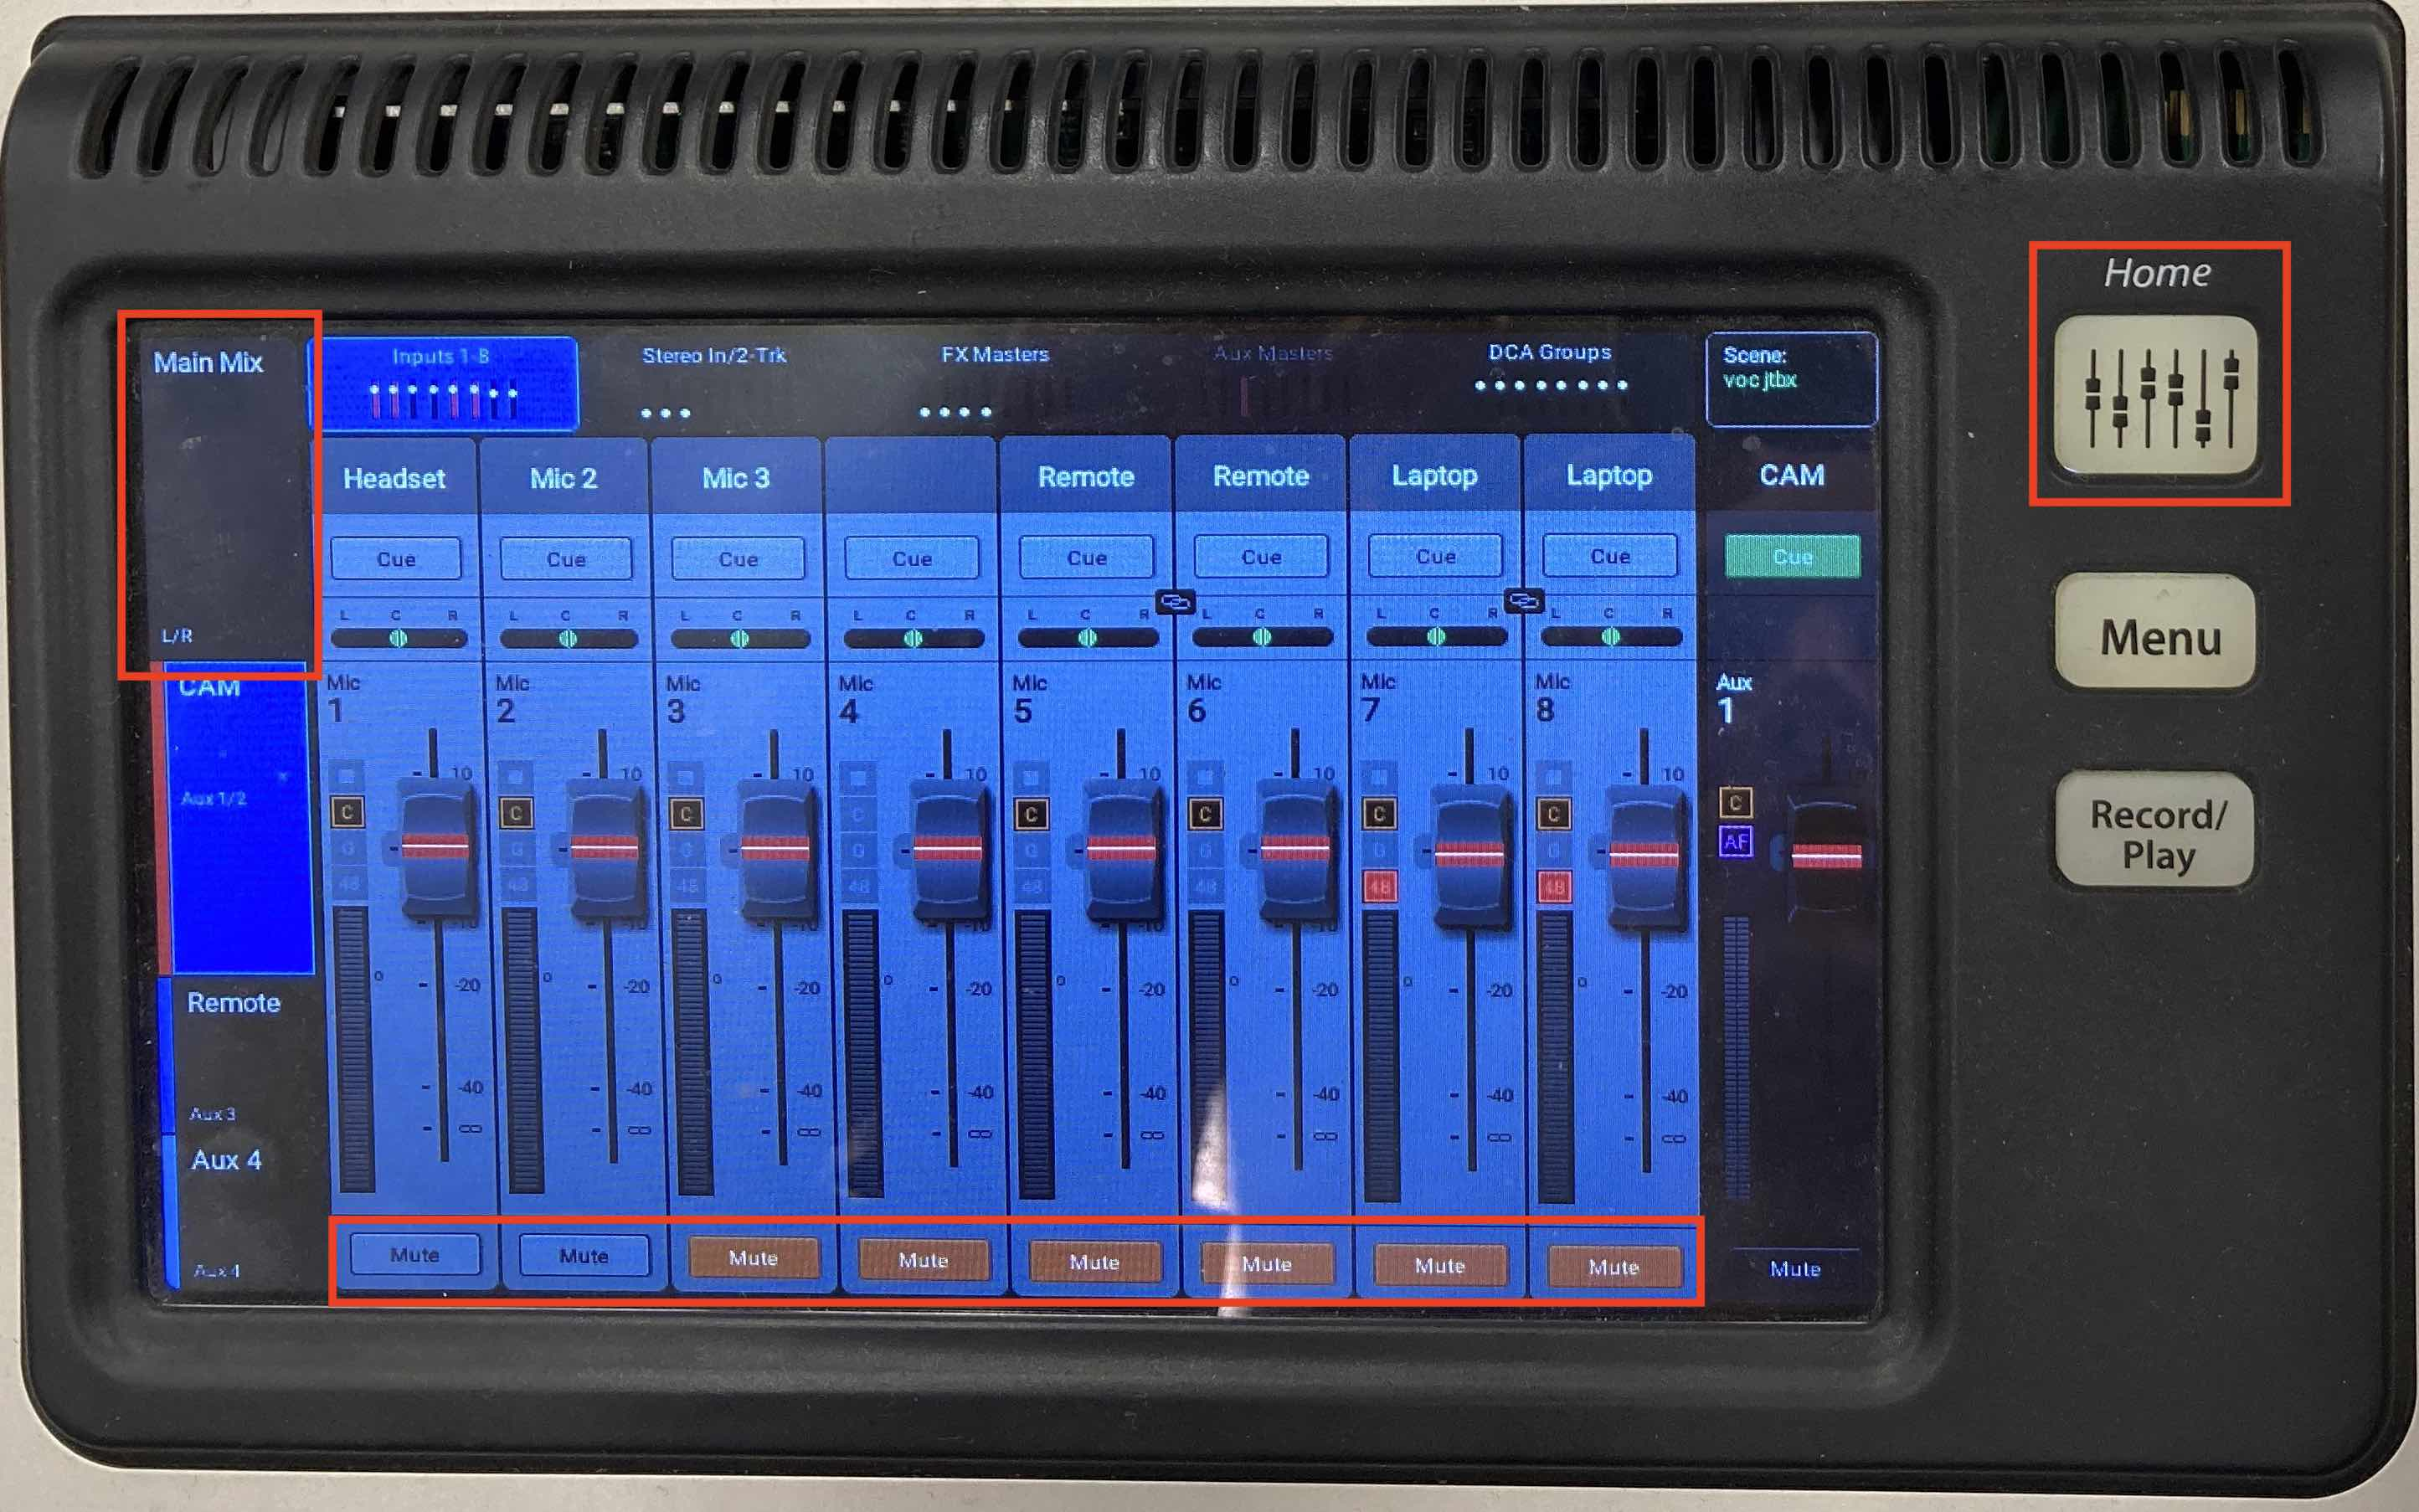
\includegraphics[width=0.9\textwidth]{images/touchmix-cam-controls.jpeg}
			\caption{Touchmix Second Page}
		\end{figure}
		\column{0.4\textwidth}
		\begin{itemize}
			\item If mute buttos are yellow, go back to "Main Mix" page
			\item If anything else is shown, just pres "Home" button
		\end{itemize}
	\end{columns}
\end{frame}

\begin{frame}{Audio Mixer Controls: Headphones}
	\begin{columns}[T,onlytextwidth]
		\column{0.6\textwidth}
		\begin{figure} 
			\centering
			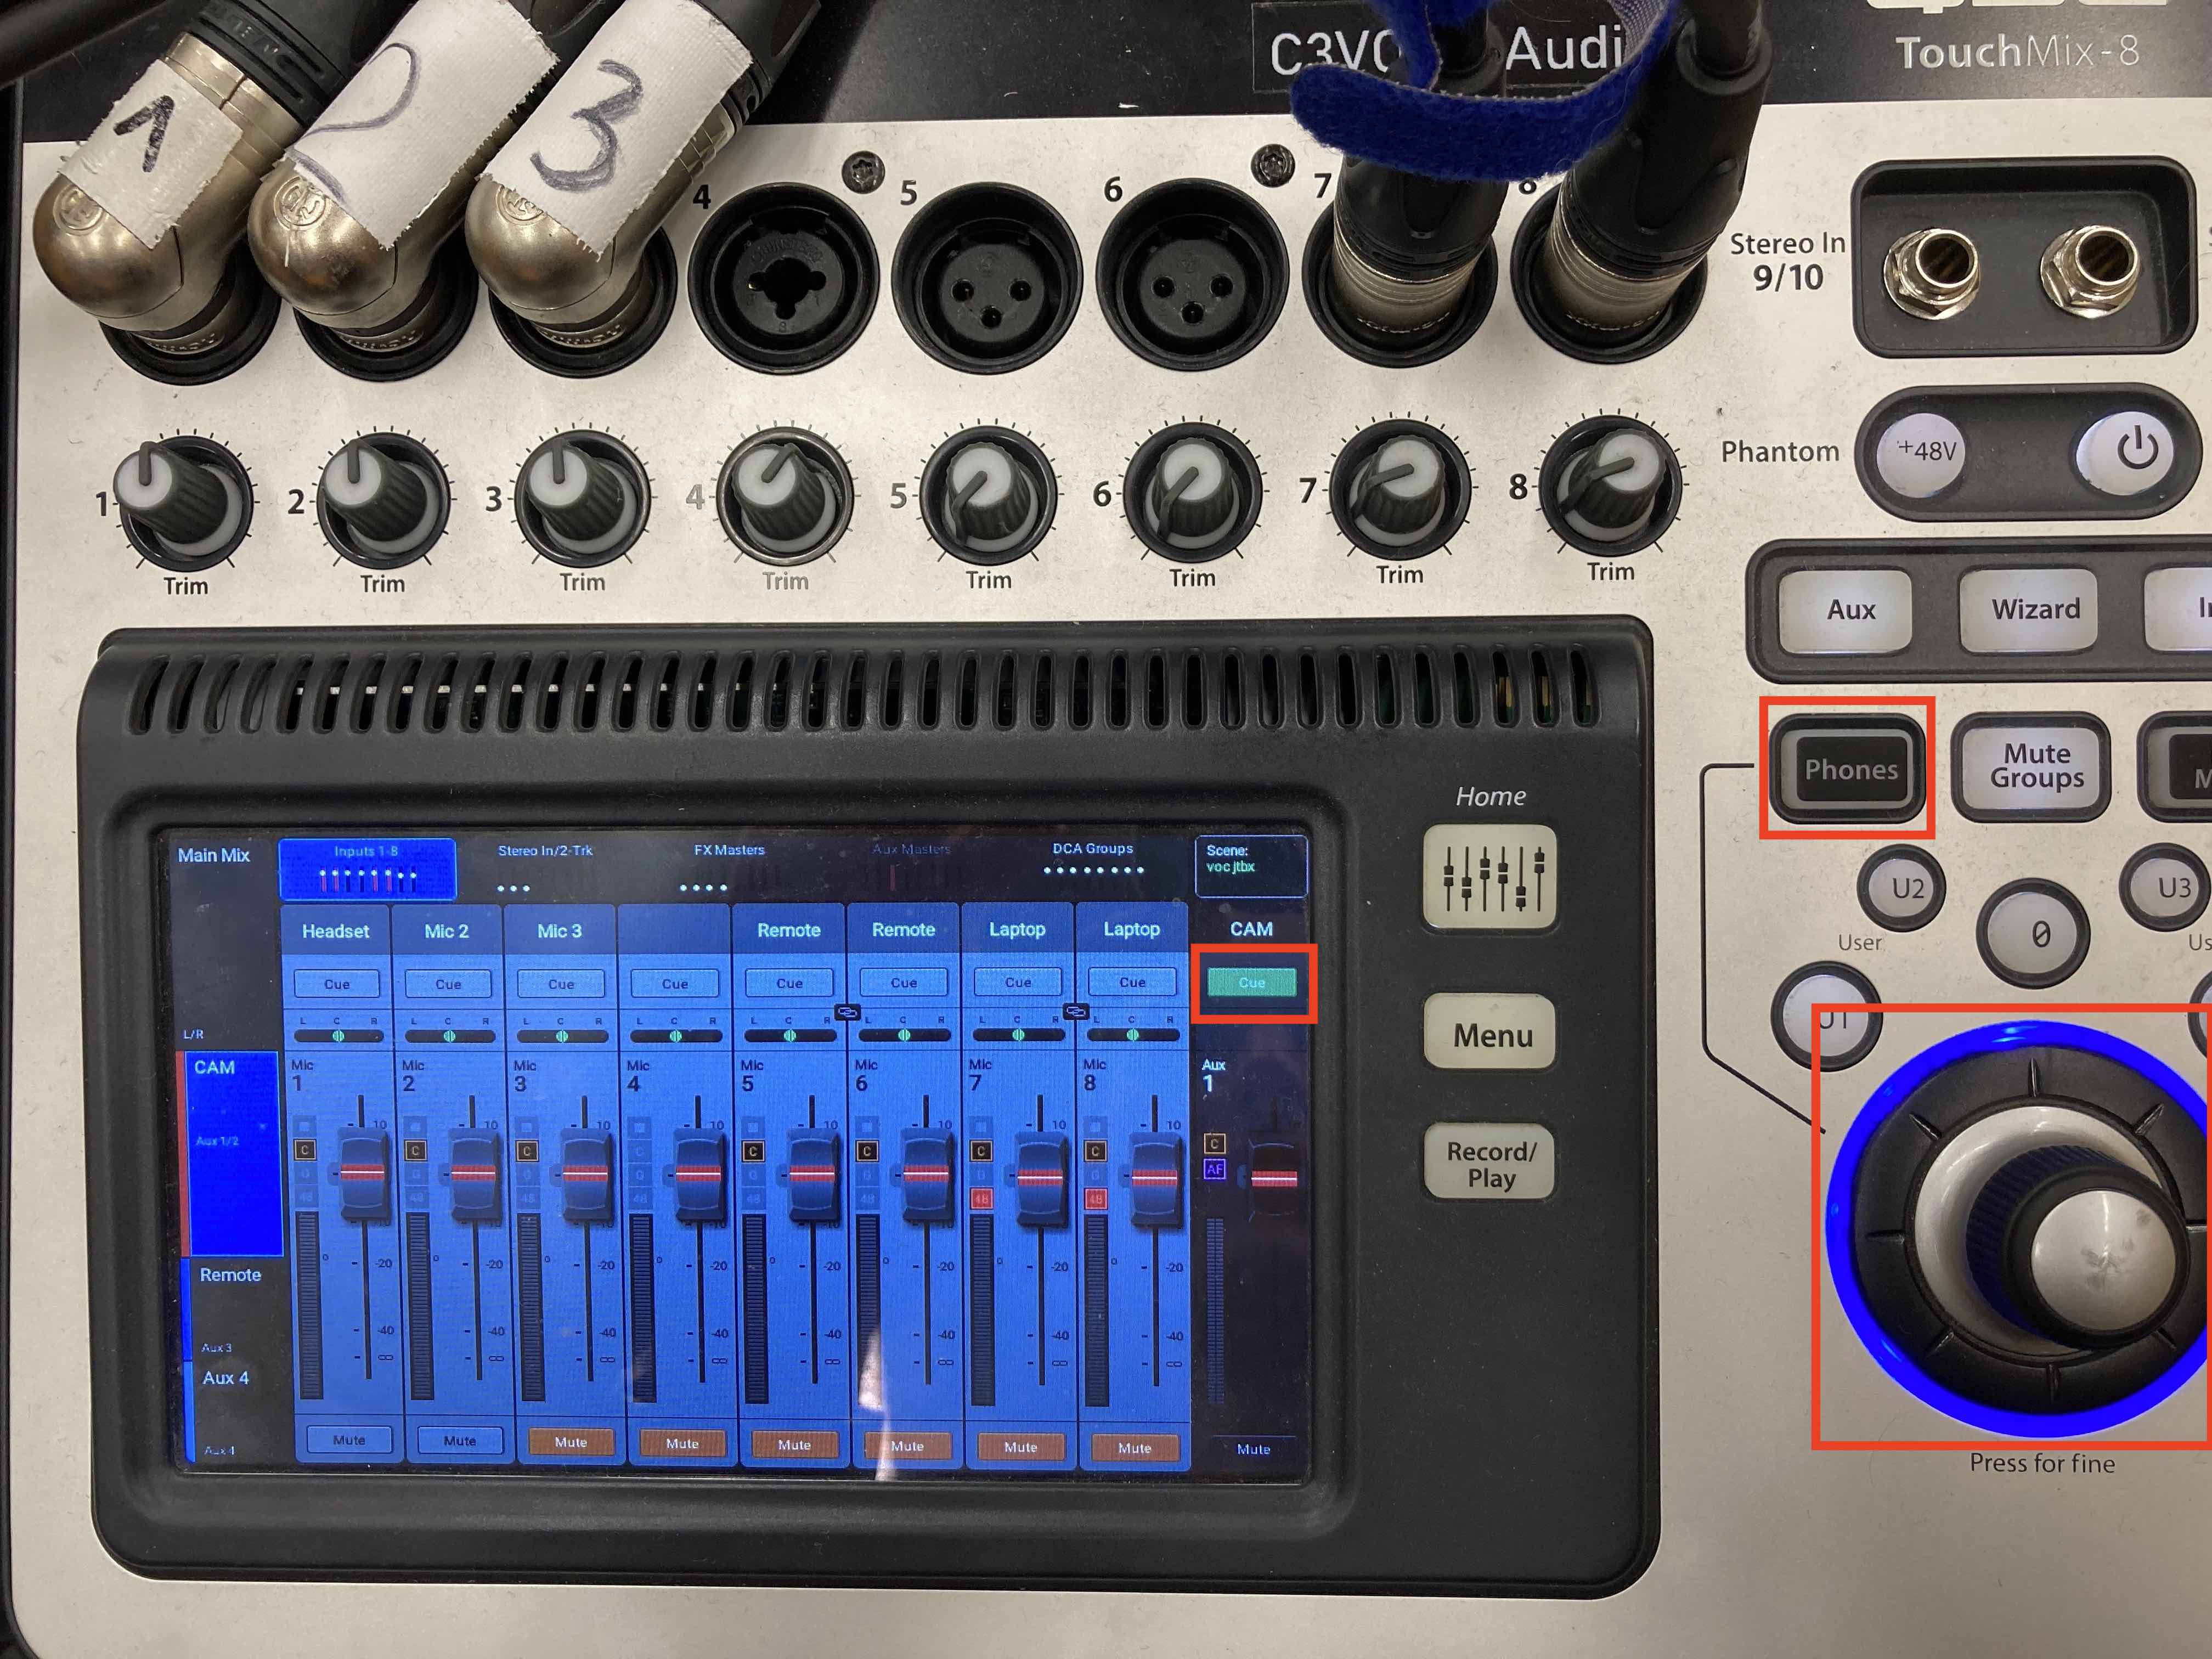
\includegraphics[width=0.9\textwidth]{images/touchmix-cam-headphones.jpg}
			\caption{Touchmix Headphones}
		\end{figure}
		\column{0.4\textwidth}
		\begin{itemize}
			\item Press "Phones" to adjust headphone loudness
			\item "Cue" on Camera/ Recoding mix must be selected
			\item Rotary knob can be used to adjust selected parameter (headphone level, channel level, etc.)
		\end{itemize}
	\end{columns}
\end{frame}

% !TEX root = ../main.tex

\begin{frame}{Microphones}
	\begin{itemize}
		\item We prefer headset microphones over handheld for speakers
		\item Distance to mouth will be constant -> more consistent audio level
		\item Handheld microphones for heralds and Q\&A
		\item Our transmitters also have a mute button (yellow light = muted)
		\item Please check battery level from time to time
	\end{itemize}
\end{frame}

\begin{frame}{Headset Placement}
	\begin{columns}[T,onlytextwidth]
		\column{0.6\textwidth}
		\begin{figure} 
			\centering
			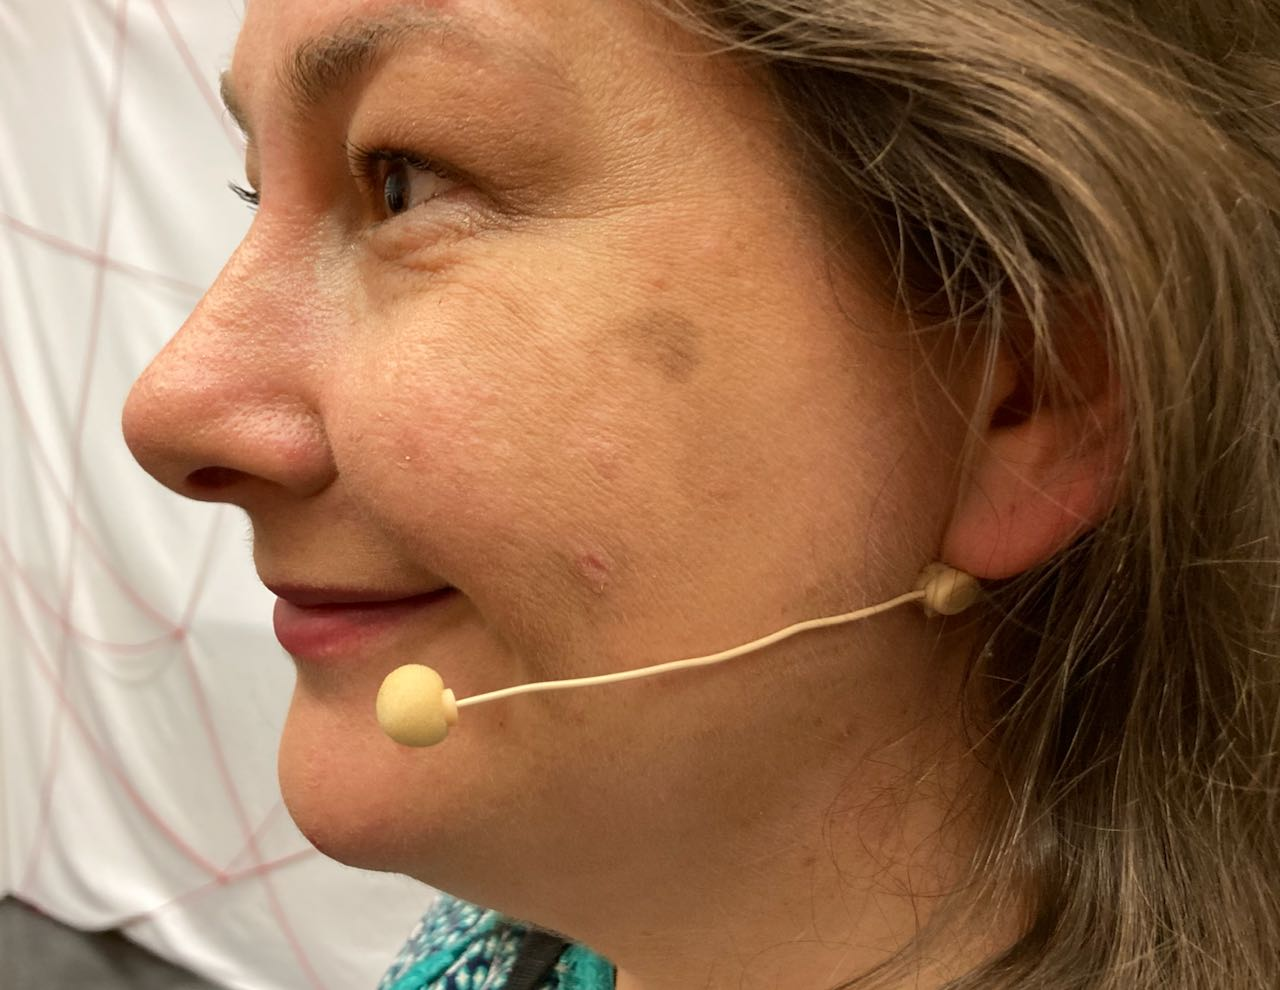
\includegraphics[width=0.9\textwidth]{images/headset-side.jpeg}
			\caption{Good headset microphone placement}
		\end{figure}
		\column{0.4\textwidth}
		\begin{itemize}
			\item Microphone shall be at the corner of the mouth
			\item Boom can slide back and forth
			\item If too far in front, there will be too much wind noise
			\item Distance to face: About 2 cm
			\item Bend boom carefully
		\end{itemize}
	\end{columns}
\end{frame}


\section{Next Steps}
\begin{frame}{Hands-On Training}
	\begin{itemize}
		\item Please do hands-on training!
		\begin{itemize}
			\item You have to try out voctomix to know its quirks
			\item Feel free to try things in a break between talks
		\end{itemize}
		\item VOC A/V-Techs are there to help you
	\end{itemize}
\end{frame}

\end{document}
